\documentclass[a4paper,12pt]{article}
\usepackage{pgfplots}
\usepackage{lmodern}
\usepackage{amssymb,amsmath}
\usepackage{ifxetex,ifluatex}
\usepackage{enumitem}
\usepackage{csvsimple,longtable,booktabs}
\usepackage{fixltx2e} % provides \textsubscript
\ifnum 0\ifxetex 1\fi\ifluatex 1\fi=0 % if pdftex
  \usepackage[T1]{fontenc}
  \usepackage[utf8]{inputenc}
\else % if luatex or xelatex
  \ifxetex
    \usepackage{mathspec}
  \else
    \usepackage{fontspec}
  \fi
  \defaultfontfeatures{Ligatures=TeX,Scale=MatchLowercase}
\fi
% use upquote if available & for straight quotes in verbatim environments
\IfFileExists{upquote.sty}{\usepackage{upquote}}{}
% use microtype if available
\IfFileExists{microtype.sty}{%
\usepackage{microtype}
\UseMicrotypeSet[protrusion]{basicmath} % disable protrusion for tt fonts
}{}
\usepackage{hyperref}
\hypersetup{unicode=true,
            pdfborder={0 0 0},
            breaklinks=true}
\urlstyle{same}  % don't use monospace font for urls
\usepackage{longtable,booktabs}
\usepackage{graphicx,grffile}
\makeatletter
\def\maxwidth{\ifdim\Gin@nat@width>\linewidth\linewidth\else\Gin@nat@width\fi}
\def\maxheight{\ifdim\Gin@nat@height>\textheight\textheight\else\Gin@nat@height\fi}
\makeatother
% Scale images if necessary, so that they will not overflow the page
% margins by default, and it is still possible to overwrite the defaults
% using explicit options in \includegraphics[width, height, ...]{}
\setkeys{Gin}{width=\maxwidth,height=\maxheight,keepaspectratio}
% Make links footnotes instead of hotlinks:
\renewcommand{\href}[2]{#2\footnote{See \texttt{\url{#1}}}}
\providecommand{\tightlist}{%
  \setlength{\itemsep}{0pt}\setlength{\parskip}{0pt}}
% Redefines (sub)paragraphs to behave more like sections
\ifx\paragraph\undefined\else
\let\oldparagraph\paragraph
\renewcommand{\paragraph}[1]{\oldparagraph{#1}\mbox{}}
\fi
\ifx\subparagraph\undefined\else
\let\oldsubparagraph\subparagraph
\renewcommand{\subparagraph}[1]{\oldsubparagraph{#1}\mbox{}}
\fi

\date{}


%
% Line Spread, Page Markings & Hyperlinked Documents
%
\linespread{1.3}
% Margin:
\usepackage[top=1.5in, bottom=1.5in, right=1in, left=1in]{geometry}

% To silence too small headheight warning
\setlength{\headheight}{15pt}

% Header & Footer:
\usepackage{fancyhdr}
\pagestyle{fancy}
\fancyhf{} % Clear all header and footer fields
\fancyhead[LO,RE]{Helpdesk Ticketing System\\{\vspace{-2pt}\scriptsize Semester 1}}
\fancyhead[LE,RO]{\leftmark\\{\vspace{-4pt}\scriptsize SWE40001 Software Engineering Project}}
\fancyfoot[LE,RO]{\thepage\ifodd\value{page}\else\hfill\fi}
\usepackage{float}

\begin{document}

{
\setcounter{tocdepth}{3}
\tableofcontents
}
\newpage
\section{Introduction}\label{introduction}

\subsection{Purpose of this document}\label{purpose-of-this-document}

This document is designed to capture and discuss, the key processes and
outcomes of the Doubtfire Helpdesk Ticketing System. This document will
outline (1) how the system is designed to function, (2) how the system
will effect stakeholders, as well as to assist the designers and
developers of the system in the development of the project. It should be
a reference of the development methodology chosen, which is outlined in
the SDLC plan document.

\textbf{Disclaimer:} This document serves as a \emph{guide} to the
development process which will be conducted throughout this final year
project. Granted the agile methodology adopted and user-centric design
process, there may be significant alterations between the content
outlined in this document and the final outcome itself. This is an
understandable consideration considering that requirements will change
as development continues, given the feedback provided from the client at
the end of sprints. This has been understood by the client and product
owner of the system.

\subsection{Background}\label{background}

\subsubsection{Swinburne University Programming
Helpdesk}\label{swinburne-university-programming-helpdesk}

The Programming Helpdesk has been offering programming assistance to
students in their first and second year of programming for many years.
Over time, as the number of subjects supported by the helpdesk grows,
the helpdesk has become busier, and as a result, it is very difficult
for tutors working at the helpdesk to keep track of who they have seen,
who still needs help and so on.

\subsubsection{Doubtfire Learning Management
System}\label{doubtfire-learning-management-system}

Doubtfire is an open source learning management system currently in use
across multiple subjects at Swinburne University of Technology and other
universities in Australia. It's used by many staff and students on a
daily basis. It provides students a simple and easy place to manage
their unit, manage where and when they upload work, and is the place in
which they receive feedback from their tutors for their submitted work.

\subsection{Key Project Personnel}\label{key-project-personnel}

\subsubsection{Client}\label{client}

The client for this project is Andrew Cain, as he oversees the running
of the helpdesk and is the administrator of Doubtfire at Swinburne
University. He is also a primary collaborator of Doubtfire.

\subsubsection{Stakeholders}\label{stakeholders}

\begin{itemize}
\tightlist
\item
  The \textbf{Project Client}, Andrew Cain (\texttt{acain@swin.edu.au})
\item
  The \textbf{Project Supervisor}, Graham Farrell
  (\texttt{gfarrell@swin.edu.au})
\item
  \textbf{Teaching staff} and \textbf{students} in any unit that
  utilises Doubtfire as the primary learning management system used for
  marking and providing feedback to students.
\item
  \textbf{Swinburne University of Technology ITS} which hosts Doubtfire
  and maintains server-side hardware.
\end{itemize}

\subsubsection{Project Manager}\label{project-manager}

\textbf{Andrew Cain} (\texttt{acain@swin.edu.au}) is the product owner
and also a primary developer to the Doubtfire learning management
system.

\subsubsection{Project Members}\label{project-members}

Refer to the
\href{https://github.com/final-year-project/documentation/wiki/Group-Contact-Details}{Group
Contact Details} of this portfolio.

\section{Terms of Reference}\label{terms-of-reference}

\subsection{Goals}\label{goals}

The Doubtfire Helpdesk Ticketing System has very clear goals which were
arrived at through use of the system, and through interviews with the
client. The system is intended to provide an simple, non-obtrusive way
in which students can create a ``ticket'' when they are physically at
the helpdesk, at this point tutor's should receive seamless
notifications regarding their updated tickets, so that they know who and
when they need to assist students who have open tickets.

The system needs to be integrated with Doubtfire for authentication and
validation purposes, as well as mobile apps for the tutors so they can
continue being mobile while working at the helpdesk.

The intended user group of the system are tutors and students working
and seeking assistance at the Programming Helpdesk.

\subsection{Objectives}\label{objectives}

\begin{enumerate}
\tightlist
\def\labelenumi{\arabic{enumi}.}
\item
  Doubtfire should be extended to provide a in which to manage open and
  closed tickets created by students
\item
  Doubtfire should be extended to provide a way to inform all users at
  the helpdesk information regarding the current status of the queue
  (such as a projection onto a whiteboard with the current queue)
\item
  Doubtfire should be extended to collect analytics of the use of the
  Ticketing System, as well as open and closed tickets
\item
  Mobile Apps should be developed for tutors while working at the
  helpdesk so that they can have access to their tickets on the go
\item
  The helpdesk should be fitted with bluetooth beacons in order to
  ensure users of the system are physically at the location of the
  helpdesk
\end{enumerate}

\subsection{Scope}\label{scope}

\begin{itemize}
\tightlist
\item
  This system will only be used at Swinburne with direct access to the
  current Doubtfire system.
\item
  The system will only be used by tutors at Swinburne, with direct
  support from the development team if needed.
\item
  The system will be developed alongside current development of the
  Doubtfire project in order to support any API needs.
\item
  The system will be developed and supported on Swinburne provided
  infrastructure such as servers and devices.
\end{itemize}

\subsection{Critical Success Factors}\label{critical-success-factors}

\textbf{CSF1:} A basic form of the system is to be rolled out to the
helpdesk for use at the completion of the project.

\emph{Basic} here is referring to the `barebones' ticketing system, that
is, using the new system:

\begin{itemize}
\tightlist
\item
  Can students continue to receive assistance at the helpdesk?
\item
  Can tutors continue to manage and supply assistance at the helpdesk?
\end{itemize}

\textbf{CSF2:} Have the system running on the existing Doubtfire
infrastructure, the Rails server. If this basic form of the system
cannot be rolled out at the completion of the unit, the project will be
deemed a failure.

\textbf{CSF3:} The system can collect and present analytical data to the
unit conveners regarding use of the Ticketing System and the Helpdesk.

\subsection{Acceptance Criteria}\label{acceptance-criteria}

Upon delivery, an acceptable product will need to demonstrate the
ability to perform the following functional tasks:

\subsubsection{Convenors}\label{convenors}

A convenor of a unit that employs Doubtfire within the unit that they
convene will be able to use the system to view analytics related to the
ticketing system being used at the helpdesk. Such analytics relate to:

\begin{itemize}
\tightlist
\item
  Number of tickets being opened
\item
  Number of tickets being opened by each student
\item
  Number of tickets being resolved
\item
  Number of tickets being resolved by each member of teaching staff
  working at the helpdesk
\item
  Number of tickets opened related to a unit
\item
  Number of tickets opened related to a specific task within a unit
\item
  On-peak and off-peak times for when tickets are opened
\item
  Times within the academic semester (each day and each week) when the
  helpdesk is the busiest and quietest
\end{itemize}

\subsubsection{Students}\label{students}

Student's that attend the helpdesk should be able to perform the
following:

\begin{itemize}
\tightlist
\item
  A student will be able to sign onto the Programming Help Desk upon
  arrival
\item
  A student will be able to open support tickets, where each ticket they
  open is related to a specific task within a specific unit that employs
  Doubtfire as a learning management system
\item
  A student will be able to close a ticket that they have opened
\end{itemize}

\subsubsection{Tutor}\label{tutor}

Tutors employed at the helpdesk should be able to perform the following:

\begin{itemize}
\tightlist
\item
  A tutor will be able to sign onto the Programming Help Desk upon the
  beginning of their shift
\item
  A tutor will be able to use the ticketing system to view current
  support tickets that have been opened by students
\item
  A tutor will be able to delegate tickets to themselves
\item
  A tutor will be able to delegate tickets to any other tutor currently
  signed on at the Programming Help Desk
\item
  A tutor will be able to close an open ticket: (a) when the issue
  associated with the ticket has been resolved and (b) when a ticket has
  been opened and should not have been
\item
  A tutor will have access to analytics related to the tickets and the
  units/tasks that the tickets are open for
\end{itemize}

\section{Establishment}\label{establishment}

\subsection{Process, Procedures and
Standards}\label{process-procedures-and-standards}

This is outlined in further detail under the
\href{https://github.com/final-year-project/documentation/wiki/SDLC-Plan}{Agile
Workflow Documentation} and
\href{https://github.com/doubtfire-lms/doubtfire-web/blob/develop/CONTRIBUTING.md}{Coding
Standards} documentation.

\subsection{Project Environment}\label{project-environment}

The physical environment of the Doubtfire Ticketing System will be at
the Helpdesk (ATC620 at Swinburne University, Hawthorn Campus). The
system operates in a room with desktop computers on each wall, running
Windows 7, and several floating tables in the middle of the room for use
with laptops.

The hardware in this room is maintained and updated by Swinburne ITS.
User accounts are managed by ITS and authentication is handled by the
SIMS system.

The server in which Doubtfire is run on
(\texttt{doubtfire.ict.swin.edu.au}) is hosted, maintained and run by
Swinburne ITS. Swinburne ITS also maintain the MySQL RDBMS which stores
confidential student information, as well as the Rails infrastructure
needed by Doubtfire.

Using the system requires:

\begin{itemize}
\tightlist
\item
  A modern desktop or mobile web browser, kept up to date. Doubtfire
  \textbf{does not support} Internet Explorer 9 or below, and is
  intended to be used by up-to-browsers such as Safari, Chrome or
  Firefox.
\item
  Any desktop or laptop running a modern operating system (Windows 10,
  OS X 10.10+, Linux distributions released within the last two years
  etc.)
\item
  Modern Android phones released in the last two years or an iPhone 5 or
  above.
\end{itemize}

\subsection{Project Team Skills
Requirements}\label{project-team-skills-requirements}

Doubtfire is both a server-side and front-end web application, where the
interface for the application is delivered through a web browser.
Proficiencies and knowledge requirements are defined as thus:

\subsubsection{API Server}\label{api-server}

Refer to the Doubtfire API
\href{https://github.com/doubtfire-lms/doubtfire-api}{README} for more
information.

\begin{itemize}
\tightlist
\item
  \textbf{\href{https://www.ruby-lang.org}{Ruby}}: The coding language
  which the server is developed in
\item
  \textbf{\href{http://rubyonrails.org}{Ruby on Rails}}: The server-side
  framework that allows Ruby code to run on a server
\item
  \textbf{\href{http://www.postgresql.org}{PostgreSQL}}: The
  object-relational database which is used during development
\end{itemize}

\subsubsection{Web Interface}\label{web-interface}

Refer to the Doubtfire Web
\href{https://github.com/doubtfire-lms/doubtfire-web}{README} for more
information.

\begin{itemize}
\tightlist
\item
  \textbf{\href{https://www.javascript.com}{JavaScript} and
  \href{http://coffeescript.org}{CoffeeScript}}: The coding language
  used to develop the front-end
\item
  \textbf{\href{http://sass-lang.com}{SCSS}}: The styling syntax used to
  style Doubtfire
\item
  \textbf{\href{http://getbootstrap.com}{Bootstrap}}: A front-end
  framework used for styling
\item
  \textbf{\href{http://angularjs.org}{AngularJS 1.4}}: A front-end
  platform designed for building web applications
\end{itemize}

\subsubsection{Additional knowledge}\label{additional-knowledge}

\begin{itemize}
\tightlist
\item
  \textbf{\href{https://git-scm.com}{Git}}: A code versioning system
  imperative to development with regards to tracking code changes and
  developer contributions
\item
  \textbf{\href{http://github.com}{GitHub}}: A website for hosting code
  repositories using Git tracking. Enables forking and pull-requests to
  merge code into the \href{http://github.com/doubtfire-lms}{official
  Doubtfire codebase}.
\item
  \textbf{\href{https://en.wikipedia.org/wiki/Representational_state_transfer}{RESTful
  architectures}}: Representational state transfer architecture styling
  which most modern web-applications are based on.
\item
  \textbf{\href{http://socket.io}{Socket.IO}}: Socket-based JavaScript
  library used to build realtime web applications.
\end{itemize}

\section{Activities, Deliverables and Capital
Resources}\label{activities-deliverables-and-capital-resources}

\subsection{Deliverables}\label{deliverables}

A functioning extension of Doubtfire which will enable students and
tutors to create and manage tickets. It will be completed using the Git
development system currently outlined in the contributing documentation
and merged into the live Doubtfire system by the client. This should
include the analytics system.

Two functioning mobile apps developed and uploaded to the respective
Apple App or Google Play stores which allows tutors to download and run
the apps.

\subsection{Activities and Tasks}\label{activities-and-tasks}

There are a number of activities that the group members must embark on
in order to ensure that the project's development and overall delivery a
success. The key activities that have been identified as critical to the
project's success are outlined and defined in detail below.

\subsubsection{Research}\label{research}

Research is absolutely imperative in terms of understanding the need for
the project and the domain for which the project is being developed for.
Research, when done correctly, provides for a concrete foundation on
which to build the project and to ensure that it is stable throughout
the entire development cycle.

Without researching the project's target domain and the functionality
that it will offer, the development would be based upon a loose
construction of ideas that vaguely resemble what purpose the product is
supposed to serve. Not only does research provide for a solid foundation
on which to develop the project, it aids in developing better problem
solving skills, critical thinking measures, confidence in what you're
developing as well as project driven motivation.

\subsubsection{Development}\label{development}

The development activity is where the knowledge gathered from the
research phase is applied and constructed into a meaningful
representation of what the project is supposed to represent. Throughout
the development phase, each group member will be completely focussed on
implementing a seamless solution.

\subsubsection{Testing}\label{testing}

A test-driven development (TDD) methodology will be adopted. This will
include testing each and all of the different tool sets that, combined,
produce the overall functionality of the ticketing system.

It is extremely important to conduct rigorous testing in order to ensure
that the product is working exactly as is intended. It is also important
to identify any issues that the system may have during the testing phase
so that these may be corrected.

\subsubsection{Documentation Authoring}\label{documentation-authoring}

After the project has been developed and tested rigorously and meets a
standard of functionality that all of the group members can agree upon,
documentation needs to be developed.

During this stage, user manuals and technical documentation will be
authored in an interactive fashion (i.e., via a Git wiki) to provide for
a complete dissection of the system and how it all works.

\subsubsection{Submission for Critical
Analysis}\label{submission-for-critical-analysis}

This task involves submitting the final project with all accompanying
documentation for critical analysis from an individual(s) separate to
the group dynamic. It is the intention of the group to have any such
individual walk away from analysing the project feeling completely
satisfied in the final product and all of the documentation provided
with it.

\subsection{Resources}\label{resources}

\subsubsection{Organisation Structure}\label{organisation-structure}

The organisation structure of the helpdesk is listed in hierachy as
thus:

\begin{enumerate}
\tightlist
\def\labelenumi{\arabic{enumi}.}
\item
  \textbf{Helpdesk Administrator}, Andrew Cain
\item
  \textbf{Helpdesk Subject Convenors}:

\begin{itemize}
\tightlist
\item
  Andrew Cain, Introduction to Programming
\item
  Alan Colman (\texttt{acolman@swin.edu.au}), Creating Web Applications
\item
  Chris McCarthy (\texttt{cdmccarthy@swin.edu.au}), Object-Oriented
  Programming
\end{itemize}

\def\labelenumi{\arabic{enumi}.}
\setcounter{enumi}{2}
\item
  \textbf{Helpdesk Subject Tutors}
\item
  \textbf{Helpdesk General Support Staff}
\item
  \textbf{Helpdesk Volunteers}
\end{enumerate}

\subsubsection{Development Equipment}\label{development-equipment}

UNIX-based systems to develop the system is required as Doubtfire does
not support development on Windows. In addition, iOS applications must
be developed using the OS X operating system, which will require the
procurement of iMacs. These can be procured through Swinburne ITS.

To test the mobile applications, an iPhone(s) will be required for the
iOS application and several Android devices will be required. Lastly
Bluetooth BLE beacons used to clock staff on and off will be required.
These can be procured through scholarships provided by Swinburne for
final year students.

\section{Risk Analysis}\label{risk-analysis}

\subsection{Risk 1}\label{risk-1}

\fbox{%
\parbox{\textwidth}{%
\begin{itemize}[label={}, leftmargin=1em]
\tightlist
\item
  \textbf{Possible Issue:} Misunderstanding or poor interpretation
  either via electronic or verbal communication
\item
  \textbf{Chance of Occurrence:} High
\item
  \textbf{Severity of Detriment to Group Ambitions:} Little to none
\item
  \textbf{Preventative Methods:}

\begin{enumerate}
\tightlist
\def\labelenumi{\arabic{enumi}.}
\item
  Ask clear and concise questions
\item
  Communicate any ideas as soon as they dawn
\item
  Document clear notes
\item
  In the event that something is not clearly communicated, make the
  issue known
\end{enumerate}
\end{itemize}
}
}

\subsection{Risk 2}\label{risk-2}

\fbox{%
\parbox{\textwidth}{%
\begin{itemize}[label={}, leftmargin=1em]
\tightlist
\item
  \textbf{Possible Issue:} The group members all have different opinions
  in regards to how a particular problem should be approached
\item
  \textbf{Chance of Occurrence:} High
\item
  \textbf{Severity of Detriment to Group Ambitions:} Low to Medium
\item
  \textbf{Preventative Methods:}

\begin{enumerate}
\tightlist
\def\labelenumi{\arabic{enumi}.}
\item
  Elect to resolve the opinion dispute by casting a majority vote
\item
  Consult the project supervisor for their opinion
\end{enumerate}
\end{itemize}
}
}

\subsection{Risk 3}\label{risk-3}

\fbox{%
\parbox{\textwidth}{%
\begin{itemize}[label={}, leftmargin=1em]
\tightlist
\item
  \textbf{Possible Issue:} Task delegation becomes an issue because no
  group member elects to take on responsibility
\item
  \textbf{Chance of Occurrence:} Medium
\item
  \textbf{Severity of Detriment to Group Ambitions:} Low to Medium
\item
  \textbf{Preventative Methods:}

\begin{enumerate}
\tightlist
\def\labelenumi{\arabic{enumi}.}
\item
  Refer to the elected responsibilities
\item
  Consult project supervisor for indisputable delegation authority
\end{enumerate}
\end{itemize}
}
}

\subsection{Risk 4}\label{risk-4}

\fbox{%
\parbox{\textwidth}{%
\begin{itemize}[label={}, leftmargin=1em]
\tightlist
\item
  \textbf{Possible Issue:} Absent from Lectures
\item
  \textbf{Chance of Occurrence:} Medium
\item
  \textbf{Severity of Detriment to Group Ambitions:} Medium to High
\item
  \textbf{Preventative Methods:}

\begin{enumerate}
\tightlist
\def\labelenumi{\arabic{enumi}.}
\item
  Always inform group members if your attendance is in jeopardy
\item
  Understand that you're an integral part to the group's success
\end{enumerate}
\end{itemize}
}
}

\subsection{Risk 5}\label{risk-5}

\fbox{%
\parbox{\textwidth}{%
\begin{itemize}[label={}, leftmargin=1em]
\tightlist
\item
  \textbf{Possible Issue:} Absent from arranged group meetings
\item
  \textbf{Chance of Occurrence:} Low
\item
  \textbf{Severity of Detriment to Group Ambitions:} Medium to High
\item
  \textbf{Preventative Methods:}

\begin{enumerate}
\tightlist
\def\labelenumi{\arabic{enumi}.}
\item
  Always inform group members if your attendance is in jeopardy
\item
  Understand that you're an integral part to the group's success
\item
  Clearly communicate any commitment issues with fellow group members
\end{enumerate}
\end{itemize}
}
}

\subsection{Risk 6}\label{risk-6}

\fbox{%
\parbox{\textwidth}{%
\begin{itemize}[label={}, leftmargin=1em]
\tightlist
\item
  \textbf{Possible Issue:} Development timelines ignored/not met
\item
  \textbf{Chance of Occurrence:} Low
\item
  \textbf{Severity of Detriment to Group Ambitions:} Severe
\item
  \textbf{Preventative Methods:}

\begin{enumerate}
\tightlist
\def\labelenumi{\arabic{enumi}.}
\item
  Understand that the group is relying on a strong work ethic to produce
  exceptional results
\item
  Constantly check your delegated tasks and review deadlines
\item
  Understand your role within the group
\item
  Understand that without submissions, the whole group suffers
\end{enumerate}
\end{itemize}
}
}

\subsection{Risk 7}\label{risk-7}

\fbox{%
\parbox{\textwidth}{%
\begin{itemize}[label={}, leftmargin=1em]
\tightlist
\item
  \textbf{Possible Issue:} Document availability issues
\item
  \textbf{Chance of Occurrence:} Low
\item
  \textbf{Severity of Detriment to Group Ambitions:} Severe
\item
  \textbf{Preventative Methods:}

\begin{enumerate}
\tightlist
\def\labelenumi{\arabic{enumi}.}
\item
  Utilise a single medium for document sharing and collaboration
\item
  Ask questions and know which tasks are delegated to each group member
\end{enumerate}
\end{itemize}
}
}

\subsection{Risk 8}\label{risk-8}

\fbox{%
\parbox{\textwidth}{%
\begin{itemize}[label={}, leftmargin=1em]
\tightlist
\item
  \textbf{Possible Issue:} Transportation issues
\item
  \textbf{Chance of Occurrence:} Low to Medium
\item
  \textbf{Severity of Detriment to Group Ambitions:} Low
\item
  \textbf{Preventative Methods:}

\begin{enumerate}
\tightlist
\def\labelenumi{\arabic{enumi}.}
\item
  Use punctuality to ensure that your transport is not jeopardised
\item
  In the event that transport is absent, communicate your situation with
  fellow group members
\end{enumerate}
\end{itemize}
}
}

\subsection{Risk 9}\label{risk-9}

\fbox{%
\parbox{\textwidth}{%
\begin{itemize}[label={}, leftmargin=1em]
\tightlist
\item
  \textbf{Possible Issue:} Delegated task not completed
\item
  \textbf{Chance of Occurrence:} Low
\item
  \textbf{Severity of Detriment to Group Ambitions:} Severe
\item
  \textbf{Preventative Methods:}

\begin{enumerate}
\tightlist
\def\labelenumi{\arabic{enumi}.}
\item
  Offer a group communication with the group member who has not produced
  material.
\item
  Involve the subject convenor and arrange a remedy.
\end{enumerate}

\end{itemize}
}
}

\section{Schedule}\label{schedule}

\subsection{Overview and Timeline}\label{overview-and-timeline}

\begin{figure}[p]
  \centering
  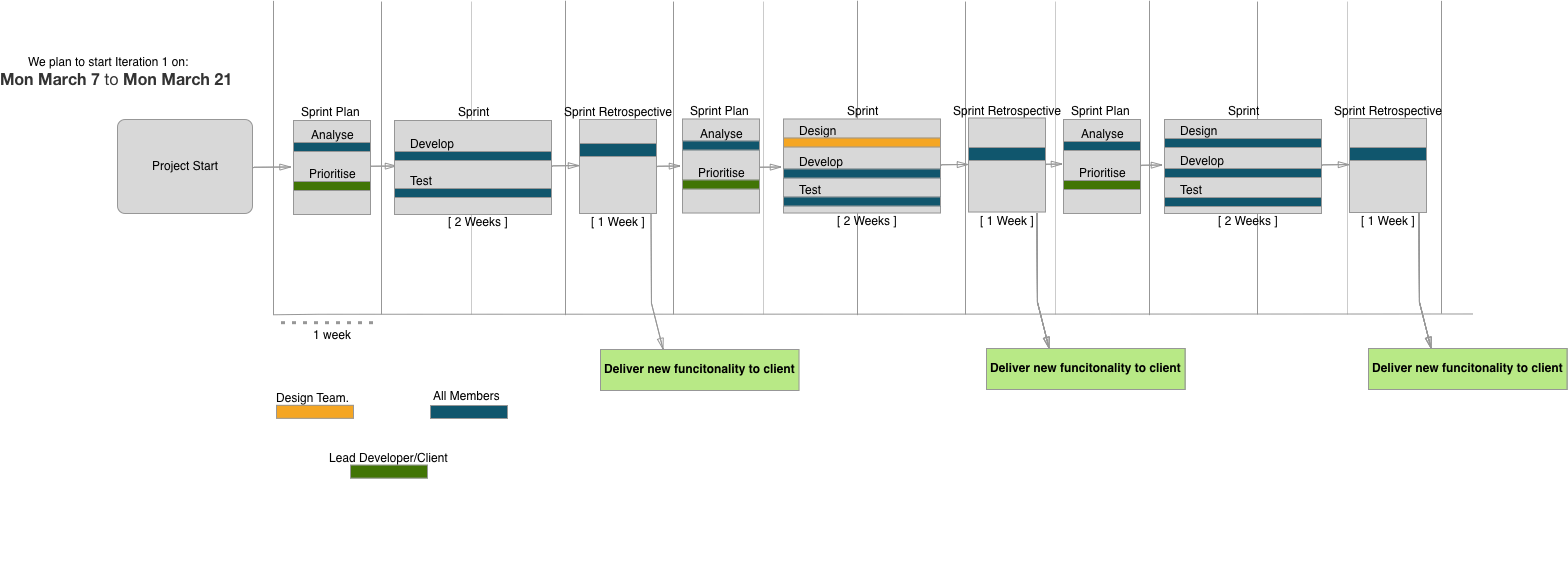
\includegraphics[width=\paperwidth, angle=90]{graph.png}
  \caption{Semesterly schedule, outlining Semester 1}
  \label{fig:schedule}
\end{figure}

An overview of the semesterly schedules are outlined in Figure ~\ref{fig:schedule}. The
team plans to adopt a fortnightly sprint, surrounded by a week of sprint
planning prior to the sprint beginning and a week of a sprint
retrospective. Further information regarding the workflow is outlined in
the
\href{https://github.com/final-year-project/documentation/wiki/SDLC-Plan}{Agile
Workflow Summary}.

The overarching plan for deliverables will occur during a Sprint
Retrospective. Within the Sprint Retrospective, work from the previous
sprint is shown to the client, which serves as a feedback loop for the
previous two-week iteration.

Thus, the general principle will be to:

\begin{enumerate}
\tightlist
\def\labelenumi{\arabic{enumi}.}
\item
  Plan a sprint, deciding which tasks need to be allocated
\item
  Work on each task over a two-week sprint
\item
  Deliver new functionality to the client during the retrospective week
\item
  Improve upon the product given the client's feedback and work on this
  for the following week.
\end{enumerate}

Whilst the dates are time-fixed, the durations of sprints, sprint
planning and sprint retrospectives are \emph{dynamic}, and so dates may
not be adhered to concretely since they only act to serve a guide. For
example, there may be a time where a two-week sprint is simply not
enough time given the time allowed, and thus, the two-week schedule may
be extended to a three or four week schedule, reducing planning and
retrospective time.

This is chiefly due to external dependencies on the project, especially
since the technical requirements will be forever changing with client
demands.

\subsection{External Dependencies}\label{external-dependencies}

\subsubsection{Client and Helpdesk
Manager}\label{client-and-helpdesk-manager}

As Andrew Cain is the lead developer for Doubtfire, and he is also the
manager of the Programming Help Desk, his decisions, choices and
influences largely sway the direction of the project.

The team will be working closely with Andrew to ensure that he and the
team always stay on the same page in terms of the project. In an agile
context, the team will conduct weekly `catch up' meetings which act,
serving as the stand-ups the team involves the client in.

\subsubsection{Other Studies}\label{other-studies}

Other final year subjects have large amounts of work during assessment
times, which will sometimes overlap with development of the project.

\subsubsection{Personal Life}\label{personal-life}

This includes general physical and mental health of each team member,
which is obviously more important than any work.

\subsection{Assumptions Made}\label{assumptions-made}

Completion of the project assumes that the relevant Swinburne services
will aid us. ITS is to provide software and hardware required to run the
system, and will also provide developmental resources as outlined in the
previous sections. It is also expected that Swinburne will aid the team
by providing the team with some suitable development room, as well as
development hardware.

Another assumption made is that the helpdesk will still operate `as-is';
the need for the project is still relevant throughout the year. There
will be no unexpected downtime of the helpdesk or indeed the University.

\section{Budget}\label{budget}

The breakdown of hours have based on worklog hours. Both the semesterly
estimates, and actual recordings are for Semester 1 are given in Table~\ref{tab:breakdown1}. The
sprint hours allocated for this semester have been indicated also, as visualised
in Figure~\ref{fig:breakdown2} from data shown in Table~\ref{tab:breakdown2}.

Estimates for the project have been calculated as thus:

\begin{enumerate}
\tightlist
\def\labelenumi{\arabic{enumi}.}
\item
  96 hours minimum allocated for project work, either performed
  individually or together
\item
  24 hours minimum allocated for team and client meetings
\item
  12 hours minimum allocated for supervisor meetings
\end{enumerate}

This gives a total of 132 hours per semester.

% \begin{figure}
%   \begin{tikzpicture}
%   \begin{axis}
%     \addplot table [x=a, y=c, col sep=comma] {semester-hours.csv};
%   \end{axis}
%   \end{tikzpicture}
% \end{figure}

\begin{table}
  \centering
  \caption{Breakdown of estimated and actual hours over the semesters}
  \label{tab:breakdown1}
  \vspace{1em}
  \csvautobooktabular{semester-hours.csv}
\end{table}

\begin{figure}
  \centering
  \begin{tikzpicture}
  \begin{axis}[
    legend entries={
      Alex,
      Jake,
      Reuben,
      Lachlan
    },
    legend pos=outer north east,
    xlabel={Sprint},
    ylabel={Hours},
    minor tick num=5,
    grid=major,
  ]
    \addplot table [x=Sprint, y=Alex, col sep=comma] {sprint-hours.csv};
    \addplot table [x=Sprint, y=Jake, col sep=comma] {sprint-hours.csv};
    \addplot table [x=Sprint, y=Reuben, col sep=comma] {sprint-hours.csv};
    \addplot table [x=Sprint, y=Lachlan, col sep=comma] {sprint-hours.csv};
  \end{axis}
  \end{tikzpicture}
  \caption{Graphical representation of hours per sprint}
  \label{fig:breakdown2}
\end{figure}

\begin{table}
  \centering
  \caption{Breakdown of recorded hours for each sprint}
  \label{tab:breakdown2}
  \vspace{1em}
  \csvautobooktabular{sprint-hours.csv}
\end{table}

\end{document}
